\section{Background and Preliminaries} \label{sec:background}
%%This section reviews several key concepts for our proposed computational machine self-confidence framework. To make the concepts discussed throughout the paper concrete and provide an accessible proof-of-concept testbed in later sections, we also describe a motivating APS application example inspired by ongoing research in unmanned robotic systems.  

\subsubsection{MDP-based Planning} \label{sec:mdp}
%The diversity of factors that influence APS self-confidence requires a rich modeling approach for algorithmic assessment. 
We establish algorithmic realizations of self-confidence assessments by initially studying APS capabilities that can be modeled as Markov decision processes (MDPs). MDPs are composed of finite states and actions for the APS that partially resolve the nondeterminism in state transitions by deciding from what probability distribution $p(\cdot)$ the next state will be sampled. %%The co-existence of nondeterministic and stochastic choices in MDPs are expressive enough to account for a range of uncertainties including adversarial environmental factors and inaccuracies in execution. %%, and limitations in prior knowledge (e.g. imperfect knowledge of $p(\cdot)$).  
MDPs have well-established connections to other widely used approaches for autonomous decision-making and learning under uncertainty, such as partially observable MDPs (POMDPs) for decision-making in limited observability environments and reinforcement learning for decision-making with incomplete model information \cite{Kochenderfer2015-uu}. As such, they provide an ideal starting point for an initial analysis of self-confidence that can be generalized in future work. 

More formally, we consider generic MDP formulations of a task \task{} delegated to an APS. In an MDP framing of \task{}, the autonomous agent must find an optimal policy $\pi = u(x)$ for an MDP with dynamical state $x$ and actions $u$, such that the objective function
$U = \mathbb{E} \left[\sum_{k=0}^{\infty} \gamma^i r(x_k,u_k) \right]$ is maximized for all times $k=0,...,\infty$ --  
where $R(x_k,u_k)$ rewards (penalizes) the APS for being in (un)desirable states and taking (un)desirable actions, $\mathbb{E}[\cdot]$ is the expected value over all possible future states, and $\gamma \in (0,1]$ is a (tunable) future discount factor. 
Given any $u_k$, the state $x_k$ updates via a Markov probabilistic transition model $x_{k+1} \sim p(x_{k+1}|x_{k},u_{k})$,  
i.e. $x_{i}$ is fully observed at time $i$ (no sensor noise), while transitions $i\rightarrow k+1$ have random perturbations.
In a fully posed MDP, $\pi$ is the optimal state-action policy, which can be recovered from Bellman's equation via dynamic programming. 
However, in many practical cases, policy approximations $\tilde{\pi}$ are required to cope with complex or uncertain dynamics (e.g. for reinforcement learning or very large state spaces) \cite{Kochenderfer2015-uu}. 
    
    
	\begin{figure}[t]%[htbp]
    	\centering
     	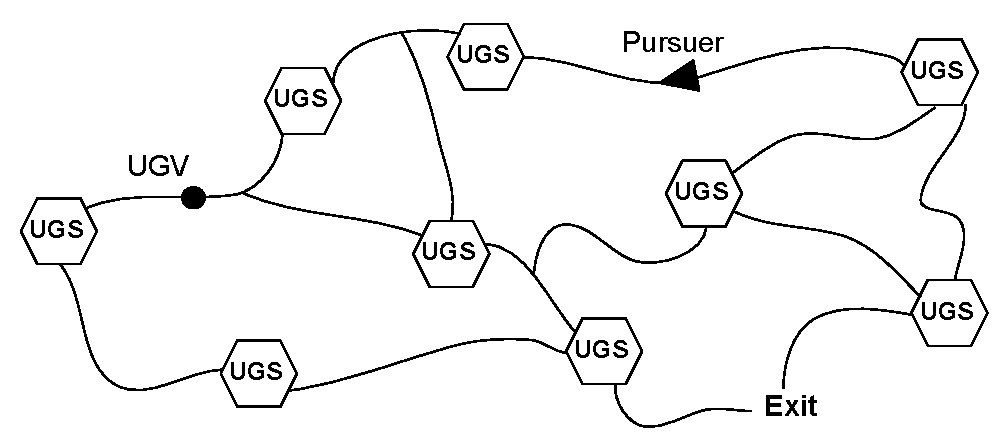
\includegraphics[width=0.5\textwidth]{Figures/RoadNet}
    	\caption{ADT in road network evading MG with information from noisy UGS.} 
        \label{fig:RoadNet}
        \vspace{-0.2cm}
    \end{figure}    
    
\subsubsection{Donut Delivery Application} \label{sec:donut_delivery}
Consider a concrete grounding example called the `Donut Delivery' problem (based on a `VIP escort' scenario~\cite{Humphrey2012-lr}). As shown in Fig.~\ref{fig:RoadNet} , an autonomous donut delivery truck (ADT) navigates a road network in order to reach a delivery destination while avoiding a motorcycle gang (MG) that will steal the donuts if they cross paths with the delivery truck. The motorcycle gang's location is unknown but can be estimated using intermittent updates from unmanned ground sensors (UGS). The delivery truck's decision space involves selecting a sequence of discrete actions (i.e. go straight, turn left, turn right, go back, stay in place). The ADT motion, UGS readings, and MG behavior are stochastic, and the problems of decision making and sensing are strongly coupled: some trajectories through the network might allow the ADT to localize the MG before heading to the delivery destination but incur a high time penalty); other trajectories may afford rapid delivery with high MG location uncertainty but increase the risk of getting caught by the MG, which can take multiple paths. A human supervisor monitors the ADT during operation. The supervisor does not have detailed knowledge or control of the ADT---but can interrogate its actions, and (based on whatever limited amount of information is provided to the supervisor) can provide `go' or `no go' commands to proceed with or abort the delivery operation before it commences. 
%, as well as potentially modify its decision making stance (`aggressively pursue exit' vs. `be very conservative and cautious') in order to better cope with the MG (which is sporadically observed and follows an unknown course). \nisar{modify last sentence -- just state go/no go?}

The physical states describing the combined motion of the ADT (whose states are always perfectly observable) and MG can be discretized in time and space to produce a Markov process model defined by some initial joint state probability distribution and joint state transition matrix, which depends on the steering actions taken by the ADT. 
%The probability of obtaining `detection' and `no detection' data from each UGS given the true state of the MG can be modeled and used to update probabilistic beliefs about the MG's state. 
%Finally, 
A reward function $R(x_k,u_k) = R_k$ can be specified for each time step $k$ to encode user preferences over the combined state of the ADT and MG, e.g. $R_k = -200$ for each time step the ADT is not co-located with the MG but not yet at the goal, $R_k= -2000$ if the ADT and MG are co-located, and $R_k=+2000$ if the ADT reaches the goal without getting caught. 
%Given these elements, the ADT's navigational planning and decision-making problem may be generally formulated as a POMDP. 
%If the MG's state is fully observable at each step $k$ (e.g. due to very reliable and accurate UGS that cover all areas of the road network), the problem reduces to an MDP. 
If the MG's state is observable at each step $k$ (e.g. due to very reliable and accurate UGS that cover all areas of the road network), the ADT's planning problem can be framed as an MDP. 

